% CV.tex
% !TEX TS-program = pdflatex
% !TEX encoding = UTF-8 Unicode
\documentclass[9pt, oneside, a4paper, titlepage]{extarticle}

\usepackage[most]{tcolorbox}
\usepackage{tikz}
\usepackage{graphicx}
\usepackage[]{geometry}
\usepackage{booktabs}
\usepackage{setspace}
\usepackage{multicol}
\usepackage{hyperref}
\geometry{
    a4paper,
    left=0.1cm,
    right=0.1cm,
    top=0.2cm,
    bottom=0.1cm
    }
    \renewcommand{\baselinestretch}{0.95}
    \definecolor{titleBack}{RGB}{0,128,255} % Blue
    
    \title{Tobias SAVARY}
    \date{}
    
    \begin{document}

    % Create the rectangle at the top of the CV 
    \tcbset{colframe=gray!95!black, colback=titleBack, arc = 3mm}
    \begin{tcolorbox}
        % Use to fill in the top
        % Affichage de l'image 
        \begin{minipage}{0.3\linewidth}
            %This is the place for the picture of your face
            % \hspace*{-0.3cm}\includegraphics[scale = 0.5]{img/TOBIAS SAVARY Photo identité Oct2020.jpg}
            \hspace*{1cm} % Permet de déplacer l'image vers la droite
            \begin{tikzpicture} 
                \begin{scope}
                    \clip [rounded corners=.5cm] (0,0) rectangle coordinate (centerpoint) (3.5,5cm); 
                    \node [inner sep=0pt] at (centerpoint) {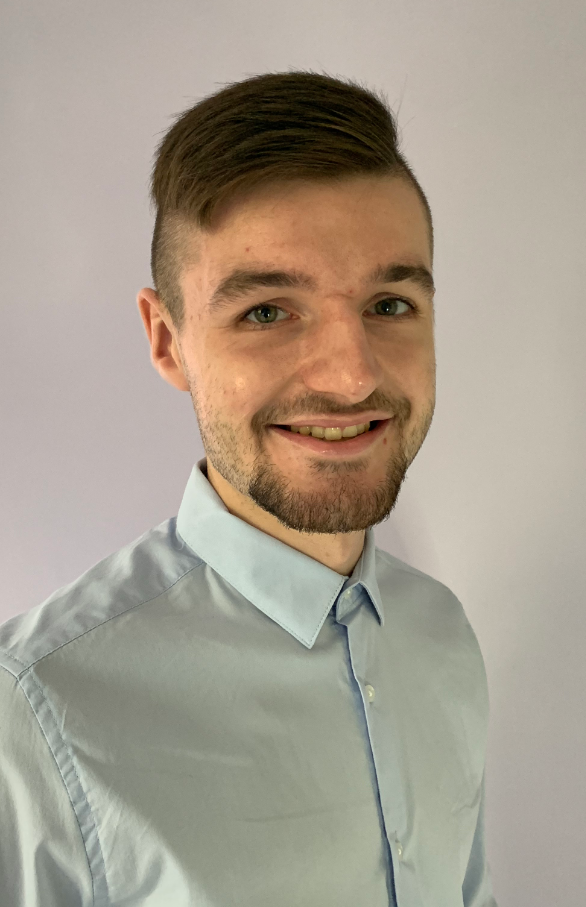
\includegraphics[width=3.5cm]{img/PhotoCV.png}}; 
                \end{scope}
            \end{tikzpicture}
        \end{minipage}%
        \hspace{1cm}%%
        \begin{minipage}{0.5\linewidth}
            % Titre du CV
            \begin{center}
                \Huge{\textcolor{white}{Tobias SAVARY}} \\
                \vspace*{0.5cm}
                % Ajouter : Cherche un stage de 6 mois Sept 2023
                \Large{\textcolor{white}{Looking for a 6-month internship as an \\engineer assistant in September 2023 \\
                \vspace*{0.5cm}
                \Large{\textcolor{white}{\emph{Student in Engeneering, Computer Science \\University of Technology of Compiègne (UTC) \\}}}
                }}
            \end{center}
        \end{minipage}%
    \end{tcolorbox}

    \tcbset{colframe=white, colback=white, arc = 2mm}
    \begin{tcolorbox}
        \vspace*{0.2cm}
        \hspace*{0.7mm}
        \begin{minipage}[t]{6.2cm}
            \begin{spacing}{0.95}
            \vspace*{-0.5cm}
            \begin{tcolorbox}[grow to left by = 0.6cm, colback = gray!25, colframe = white]
                % \section*{Profile}
                %     Here you can see my profile and I will complete it next time.
                
                \section*{\\Contact}
                \hspace*{0.4cm}
                10 Bis Rue de Château Rouge 
                \vspace*{0.2cm}
                
                \hspace*{0.4cm}
                60730 Cauvigny - France\\ \\
                \hspace*{0.4cm}
                Tel: +33 7 65 21 77 91\\
                % \vspace*{0.2cm}
                \hspace*{0.4cm}
                Email: savarytobias@hotmail.com\\

                \vspace*{0.1cm}
                \hspace*{0.4cm}\href{www.linkedin.com/in/tobiassavary}{www.linkedin.com/in/tobiassavary}
                \section*{Expertise}
                \begin{multicols}{2}
                \begin{itemize}
                    \item Python
                    \item C
                    \item C++
                    \item SQL
                    \item Ocaml
                    \columnbreak                    
                    \item Lisp
                    \item ARM
                    \item HTML
                    \item CSS
                    \item \LaTeX
                \end{itemize}
                \end{multicols}
                \vspace*{0.2cm}
                \section*{Skills}

                \begin{itemize}
                    \vspace*{0.3cm}
                    \item Comfortable use of office software (Word / Excel / Paint/ \\PowerPoint / \LaTeX \ldots)
                    \vspace*{0.2cm}
                    \item Ease of use for various mobile \\applications
                    \vspace*{0.2cm}
                    \item Mastery of programming languages : Python, C, C++, SQL, Ocaml, Lisp, ARM, HTML, CSS.
                    \vspace*{0.2cm}
                    \item Car driving license

                \end{itemize}


                \vspace*{0.2cm}
                \section*{Activities and interests}
                
                \begin{itemize}
                    \vspace*{0.3cm}
                    \item Active involvement in the communication events proposed 
                    by the school (Open House, Student Day, presentation of the 
                    training to the students of final year in the high schools of 
                    the agglomeration)
                    \vspace*{0.2cm}
                    \item Cycling and involvement in various events and sports meetings
                    \vspace*{0.2cm}
                    \item Swimming, Badminton, 
                    
                    Table Tennis.
                \end{itemize}

            \end{tcolorbox}
        \end{spacing}
        \end{minipage}
        \hspace*{0.4mm}
        \begin{minipage}[t]{12.8cm}
            \vspace*{-0.5cm}
            \begin{tcolorbox}[grow to right by = 0.6cm, colback = gray!25, colframe = white]
                \section*{Project}
                \begin{itemize}
                    \item Creation of board games with Python (Scrabble, Futoshiki)
                    \item Mathematical sets management with Ocaml
                    \item Phylogenetic tree processing, encoding and decoding of 
                    encrypted messages, image contours simplification and moving 
                    a robot in C
                    \item Coding simple web pages with HTML and CSS
                    \item Object-oriented programming in C++ : design and development of the Machi Koro board game
                    \item Design and implement a database for a veterinary clinic in SQL with a Python interface
                    \item Realization of an expert system in Lisp
                \end{itemize}
                
                \section*{Professional experience}
                \begin{itemize}
                    \item \textbf{2022 - present}: Work in the university library (Reception, promotion of digital resources, organization of events\dots)
                    \item \textbf{2022}: 2 months excellence internship in the INRIA 
                    laboratory in Grenoble in order to realize a 
                    graphical interface to develop a game for learning
                    debugging
                    \item \textbf{2021}: Professional internship in the Oise departmental services :
                    \begin{itemize}  
                        \item Multi-skilled administrative assistant -  Social Works Committee [COS60]
                        \item Multi-skilled administrative assistant - Departmental House for Handicapped Persons of the Oise [MDPH60]
                        \item Receptionist agent - Oise Departmental Housing Information Agency [ADIL60]
                    \end{itemize}
                
                    \item \textbf{2017}: Observation internship in computer science at the Digital Department of the Departmental Council
                    
                    \item \textbf{2017-2022}: Childcare and private lessons of mathematics and computer course
                \end{itemize}

                \section*{Education}
                \begin{itemize}
                    % Master degree in computer engineering expected Jul 2025
                    % Student computer engineering at the UTC expected Jul 2025
                    \item \textbf{2022}: Master degree in computer engineering expected July 2025
                    \item \textbf{2020-2022}: Preparatory training integrated into the Polytech 
                    \\ network of engineering schools, backed up by the "Mathematics 
                    and Computer Science" courses of the University of Grenoble Alpes [UGA], 
                    including cross-disciplinary courses 
                    (English, project management, professional exploration, \ldots). \emph{Ranking: 120th out of 1,564 students}
                    \item \textbf{2020}: Baccalauréat (Serie S - European section English - With Honors)
                    \item \textbf{2018}: Cambridge English Certification
                    \item \textbf{2017}: National Diploma of Brevet (With Honors)
                \end{itemize}

                \section*{Langages}
                    \begin{itemize}
                        \item French (Native speaker)
                        \item English (European B2 level),One week immersion in a host family (England)
                        \item German (European A2 level), One week of school exchange (Germany)
                         % One week of school exchange
                    \end{itemize}

                
            \end{tcolorbox}
        \end{minipage}
    \end{tcolorbox}
\end{document}